\documentclass[border=0.01cm]{standalone}

\usepackage{tikz}
\usetikzlibrary{decorations.pathreplacing}
\usetikzlibrary{shapes,decorations,arrows,calc,arrows.meta,fit,positioning}
\usetikzlibrary{shadows}
\tikzset{
    -Latex,auto,semithick,
    state/.style ={rectangle, draw, minimum width = 0.7 cm},
    point/.style = {circle, draw, opacity=1, inner sep=0.05cm, fill,node contents={}},
    bidirected/.style={Latex-Latex,dashed},
    el/.style = {inner sep=2pt, align=left, sloped}
}

\begin{document}

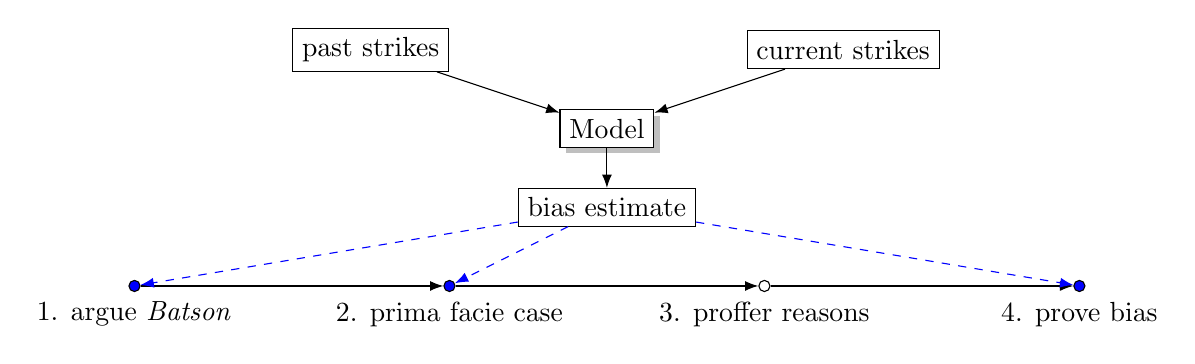
\begin{tikzpicture}
  \node (A) at (0,0) [label=below:{1. argue \emph{Batson}},point,fill={blue}];	
  \node (B1) at (4,0) [label=below:{2. prima facie case},
                       point,fill={blue}];	
  \node (B2) at (8,0) [label=below:{3. proffer reasons},
                       point, fill={white}];
  \node (B3) at (12,0) [label=below:{4. prove bias},point,fill={blue}];
   \node (M) at (6,2) [state, drop shadow, fill={white}] {Model};
   \node (PB) at (6,1) [state] {bias estimate};
    \node (H) at (3,3) [state] {past strikes};
    \node (C) at (9,3) [state] {current strikes};
    %\node (OE) at (6,-2) [state] {other evidence};

    \path (A) edge (B1);
    \path (B1) edge (B2); 
    \path (B2) edge (B3);
    \path (M) edge (PB);
    \path (PB) edge (A) [dashed, blue];
    \path (PB) edge (B1) [dashed, blue];
    \path (PB) edge (B3) [dashed, blue];
    \path (H) edge (M);
    \path (C) edge (M);
    %\path (OE) edge (B3) [red];

\end{tikzpicture}

\end{document}
